\subsection{FFT}
Se implementó la FFT utilizando el algoritmo de Cooley-Tukey de manera recursiva. Se probó con diversas entradas reales aleatorias, de tamaño 4096, con una media temporal de $40 \ \mu s$.

\subsection{Programa Principal}
Se desarrollo un programa, el cual permite agregar midis de cualquier duración, para luego sintetizar cada track desead di dicho archivo. Permite seleccionar diversos instrumentos, varios de ellos con parámetros modificables. Además, es posible compilar dichos tracks en un archivo del tipo wav y hasta generar un archivo de ``preview'' de un track dado, es decir una pequeña muestra de como se escucha un track en particular.

También es posible elegir efectos a aplicar, tanto para el archivo wav final, como para cada track en particular.

\begin{figure}[H]
	\centering
	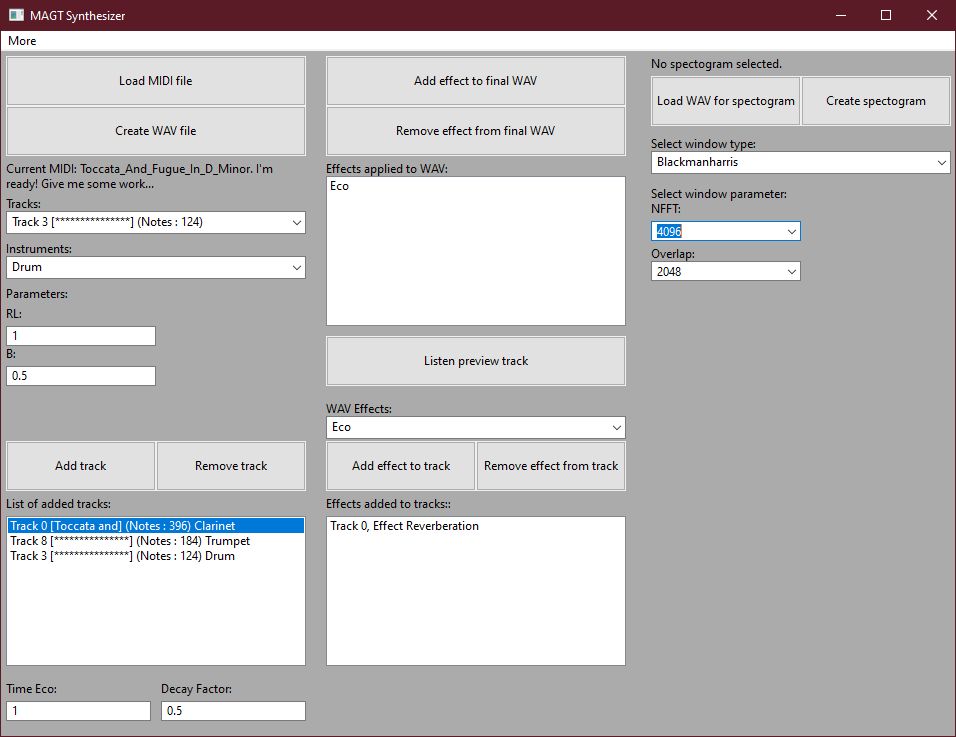
\includegraphics[width=0.8\textwidth]{ImagenesEjercicio8/GUI2.PNG}
\caption{Captura de la GUI implementada.}
	\label{fig:gui}
\end{figure}

Finalmente se destaca que es posible realizar espectrogramas de cualquier archivo wav, sea generado por este programa o no, pudiendo elegir el tipo de ventana, la cantidad de puntos de la FFT y el factor de overlap. 

Cabe destacar que el programa fue desarrollado en su totalidad en C++, a excepción de los gráficos del espectrograma, los cuales son generados mediante un llamado a un código en Python. El front-end se implementó mediante el uso de la librería WxWidgets.